\documentclass[tikz,border=4pt]{standalone}
% Shared visual grammar: role fills, dark connectors, and 7-point typography.
% Build each standalone figure from this directory. No external images required.
\pdfinfoomitdate=1
\pdftrailerid{}
\usepackage[T1]{fontenc}
\usepackage{helvet}
\renewcommand{\familydefault}{\sfdefault}
\usepackage{amsmath,amssymb}
\hyphenpenalty=10000
\exhyphenpenalty=10000
\usetikzlibrary{arrows.meta,calc,fit,positioning,decorations.pathreplacing,backgrounds}
\definecolor{ink}{HTML}{172B3A}
\definecolor{muted}{HTML}{586D85}
\definecolor{datafill}{HTML}{F1F5F9}
\definecolor{dataline}{HTML}{62748E}
\definecolor{modelfill}{HTML}{E5E9FF}
\definecolor{modelline}{HTML}{7887C7}
\definecolor{llmfill}{HTML}{FFE4E8}
\definecolor{llmline}{HTML}{E68494}
\definecolor{truthfill}{HTML}{D0FAE5}
\definecolor{truthline}{HTML}{35A782}
\newcommand{\seven}{\fontsize{7}{8.5}\selectfont}
\tikzset{
 every node/.append style={font=\seven,text=ink,align=center},
 box/.style={draw=dataline,fill=white,rounded corners=3pt,line width=.65pt,inner sep=5pt,minimum height=8mm},
 data/.style={box,fill=datafill},
 model/.style={box,draw=modelline,fill=modelfill},
 llm/.style={box,draw=llmline,fill=llmfill},
 truth/.style={box,draw=truthline,fill=truthfill},
 title/.style={font=\seven\bfseries,inner sep=1pt},
 word/.style={text=muted,inner sep=1pt,align=center},
 label/.style={fill=white,inner xsep=2pt,inner ysep=1pt,text=muted},
 flow/.style={-{Stealth[length=2.4mm,width=1.9mm]},draw=ink,line width=1.2pt,shorten >=1.5pt},
 branch/.style={-{Stealth[length=2mm,width=1.6mm]},draw=ink,line width=.9pt,shorten >=1pt},
 route/.style={draw=ink,line width=1.2pt},
 update/.style={-{Stealth[length=2.2mm,width=1.7mm]},draw=modelline,line width=1pt,dash pattern=on 3pt off 2pt,shorten >=1.5pt},
 boundary/.style={draw=dataline,dash pattern=on 3pt off 2pt,rounded corners=3pt,line width=.6pt},
 chip/.style={minimum height=4mm,inner xsep=3pt,inner ysep=1.5pt,rounded corners=2pt},
}
% Optional role key. Anchor at the center of an uncluttered final row.
\newcommand{\rolekey}[2]{
 \node[word,anchor=east] at (#1-6.6,#2) {\textit{Key}};
 \node[data,chip] at (#1-5.2,#2) {records / data};
 \node[model,chip] at (#1-1.9,#2) {learned model / policy};
 \node[llm,chip] at (#1+1.65,#2) {LLM signal};
 \node[truth,chip] at (#1+4.95,#2) {labels / evaluation};
}

\begin{document}
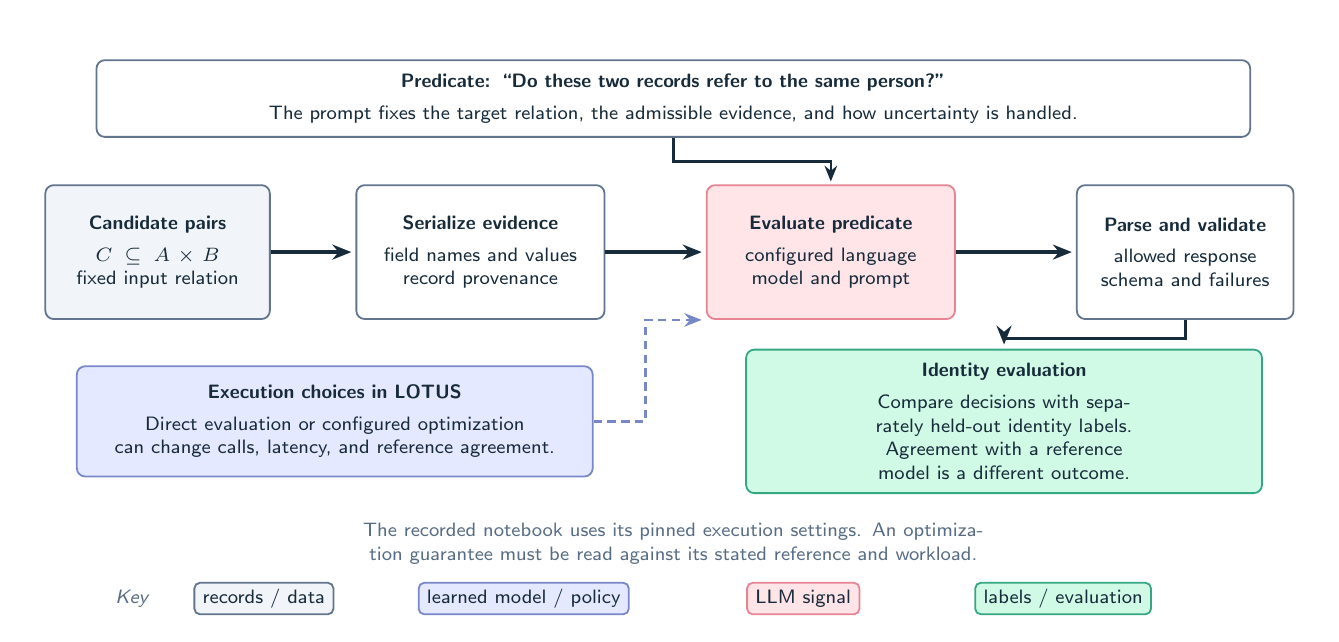
\begin{tikzpicture}

\useasboundingbox (-.2,.3) rectangle (16.1,-7.15);
\node[box,text width=143mm] (predicate) at (8,-.6) {\textbf{Predicate: ``Do these two records refer to the same person?''}\\[3pt]The prompt fixes the target relation, the admissible evidence, and how uncertainty is handled.};
\node[data,text width=25mm,minimum height=17mm] (c) at (1.45,-2.55) {\textbf{Candidate pairs}\\[3pt]$C\subseteq A\times B$\\fixed input relation};
\node[box,text width=28mm,minimum height=17mm] (serialize) at (5.55,-2.55) {\textbf{Serialize evidence}\\[3pt]field names and values\\record provenance};
\node[llm,text width=28mm,minimum height=17mm] (judge) at (10,-2.55) {\textbf{Evaluate predicate}\\[3pt]configured language\\model and prompt};
\node[box,text width=24mm,minimum height=17mm] (parse) at (14.5,-2.55) {\textbf{Parse and validate}\\[3pt]allowed response\\schema and failures};
\draw[flow] (c) -- (serialize); \draw[flow] (serialize) -- (judge); \draw[flow] (judge) -- (parse);
\draw[branch] (predicate.south) -- (8,-1.4) -| (judge.north);
\node[model,text width=62mm,minimum height=14mm] (plan) at (3.7,-4.7) {\textbf{Execution choices in LOTUS}\\[3pt]Direct evaluation or configured optimization\\can change calls, latency, and reference agreement.};
\node[truth,text width=62mm,minimum height=14mm] (audit) at (12.2,-4.7) {\textbf{Identity evaluation}\\[3pt]Compare decisions with separately held-out identity labels.\\Agreement with a reference model is a different outcome.};
\draw[update] (plan.east) -- (7.65,-4.7) |- (judge.south west);
\draw[flow] (parse.south) -- (14.5,-3.65) -- (12.2,-3.65) -- (audit.north);
\node[word,text width=143mm] at (8,-6.25) {The recorded notebook uses its pinned execution settings. An optimization guarantee must be read against its stated reference and workload.};
\rolekey{8}{-6.95}

\end{tikzpicture}
\end{document}
